\documentclass[tikz]{standalone}

\usepackage[latin1]{inputenc}
\usepackage{tikz}

% GNUPL
\begin{document}
\pagestyle{empty}


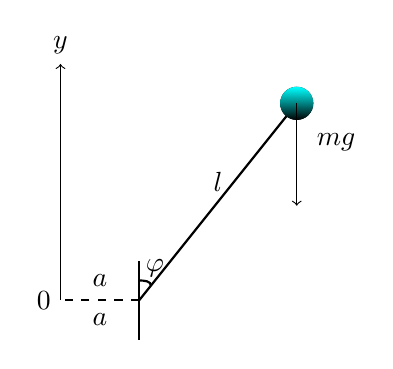
\begin{tikzpicture}
    \draw[->] (0,0) -- (0,3) node[above] {$y$};
    \draw [black, dashed, semithick] (1,0) -- (0,0);
    \draw [black, thick] (1,-0.5) -- (1,0.5);
    \draw [black, thick] (1,0) -- (3,2.5);
    \coordinate [label=left:$0$] (0) at (0,0);
    \coordinate [label=center:$a$] (3) at (0.5,0.25);
    \coordinate [label=center:$a$] (3) at (0.5,-0.25);
    \coordinate [label=center:$\varphi$] (3) at (1.2,0.4);
    \coordinate [label=center:$l$] (3) at (2,1.5);
    \coordinate [label=center:$mg$] (3) at (3.5,2);
    \draw[black,thick] (1,0.25) to [out=0,in=90] (1.15,0.18);
    \shade[top color=cyan, bottom color=black] (3,2.5) circle (6pt) [fill=black!];
    \draw [->] (3,2.5) --(3,1.2);

\end{tikzpicture}


\end{document}